\documentclass[twocolumn]{article}

%\usepackage{cleveref}
\usepackage{amsmath}
\usepackage{float}
\usepackage{graphicx}
\usepackage{caption}


% Make table names in captions boldfaced
\captionsetup[table]{labelfont=bf}
\captionsetup[figure]{labelfont=bf}

\begin{document}
%opening
\title{Mitigating the radio blackout effect of plasma sheaths at hypersonic and reentry velocities}
\author{Jack Nelson,\\
	Physics Department,\\
	Occidental College, Los Angeles, CA}
\date{October 2016}
\twocolumn[ % hacky trick to get a one-column abstract in a two-column article
	\begin{@twocolumnfalse}
		\maketitle
			\begin{abstract}
			Airborne vehicles traveling through an atmosphere at hypersonic velocities, especially in excess of Mach 15, face significant atmospheric heating that produces plasma sheaths which surround the vehicle.
			 Depending on the density of the atmosphere, the shape of the vehicle, and its speed, free electrons in the plasma attenuate and reflect incident electromagnetic waves, making communication to and from the hypersonic vehicle difficult or impossible.
			 Various methods of communicating through the plasma sheath have been proposed and studied since the early 1960's, yet a single elegant solution has not been found in unclassified research to date.
			 
			 In this paper, we will establish a theoretical overview of the problem and look at the associated plasma physics in order to better frame the potential solutions.
			 These solutions can be divided into two types: passive methods, which seek to affect the properties of the plasma sheath using passive features such the shaping of the vehicle, and active methods, which use active systems to communicate through the plasma sheath barrier.
			 We will examine some of the passive and active solutions that have been proposed, as well as recent studies which propose solving the communications blackout problem using active electromagnetic fields and $\mathbf{E}\times\mathbf{B}$ Lorentz forces.
			 A method which uses electromagnetic scattering off of resonances induced by radio signals from outside the plasma sheath is presented as a solution that has the potential to minimize weight and equipment volume in the vehicle, yet remain effective.
	 
	
			\end{abstract}
		\end{@twocolumnfalse}
	]
\section{Introduction}
	Spacecraft reentering an atmosphere from orbital velocities and aircraft traveling at hypersonic speeds experience the problem of aerodynamic heating, in which their large kinetic energies are transferred into heat by hypersonic interactions with the atmosphere.
	The problem of convective aerodynamic heating of a reentry vehicle was adequately solved by the first human space flights in the early 1960's.
	For reentry speeds, was found that blunt bodies as opposed to slender, streamlined ones minimize the total heat which is transferred to the vehicle from the air.\cite{allen_study_1958}
	Blunt body capsule designs coupled with ablative heat shield technology created a simple yet effective solution to the reentry heating problem which is still widely used today.
	For hypersonic aircraft which operate at less than reentry speeds, such as NASA's X-15 piloted research vehicle, the heating problem is solved using thick skin heat sinks made of high heat capacity superalloys such as Inconel-X.\cite{stillwell_x-15_1965}
	
	A side-effect of the hypersonic heating problem is the generation of large volumes of plasmisized atmospheric gases and the formation of a plasma sheath which envelopes the vehicle at high speeds.
	The basic properties of plasma sheaths, such as thickness, temperature, and density, are not uniform over the entire sheath, are highly dependent on the vehicle configuration and atmosphere, and are extremely difficult to accurately predict.
	
	An overview of the paper is as follows: \S\ref{sec:PlasmaSheaths} summarizes the basic properties of hypersonic vehicle plasma sheaths and introduces the plasma frequency $\omega_p$ as a fundamental measure of whether a plasma sheath will attenuate a radio wave with carrier frequency $\omega_s$.
	\S\ref{sec:Waves} gives an overview of electromagnetic waves propagating through a plasma, as well as waves in the plasma medium itself, referred to as Langmuir waves or electron acoustic waves.
	\S\ref{sec:Overview} divides a number of potential solutions to the blackout problem into active and passive methods, and briefly evaluates each one.
	\S\ref{sec:Prior} summarizes past research into the radio blackout problem and potential solutions.
	In \S\ref{sec:Solutions}, we look at a few promising solutions that have been studied in the last two decades which could potentially solve the radio blackout problem with minimal impact to the rest of a vehicle's systems and design.
	
\section{Plasma Sheaths of Hypersonic Vehicles} \label{sec:PlasmaSheaths}
In this section, we will summarize the processes by which plasma is generated by a hypersonic vehicle, as well as the characteristic properties of the plasma.
This theory, combined with the additional theory of waves in plasmas presented in \S\ref{sec:Waves}, will provide a theoretical basis to understand and evaluate solutions to the radio blackout problem.

\subsection*{Aerothermodynamics of Hypersonic Vehicles}
Vehicles traveling through an atmosphere at speeds greater than Mach 5 create strong shock waves in front of them which generates varying amounts of plasma from atmospheric gases.
The generation of this plasma, and its enveloping of the entire vehicle in a sheath, is what prevents radio signals from reaching or leaving the vehicle.

\subsection*{Properties of Hypersonic Plasma Sheaths}
Plasma is a state of matter which is characterized by free-flowing negatively-charged electrons, positive ions, and other neutral atoms and particles.
The free electrons and ions give plasma unique electromagnetic properties not seen in the other states of matter.

An important characteristic property of a plasma is its plasma frequency $\omega_p$ given in units of radians/second by the equation
\begin{equation} \label{plasma_f}
\omega_p = \sqrt{\frac{n_e e^2}{\epsilon_0 m_e}}
\end{equation}
where $e$ is the charge of the electron, $\epsilon_0$ is the permitivity of free space, and $m_e$ is the mass of the electron. 
The quantity $n_e$ is the density of electrons in the plasma.\cite{chen_introduction_1984,kim_analysis_2008}
Equation \ref{plasma_f} is interchangeably referred to as the plasma frequency and plasma electron frequency. The plasma frequency given is the resonance frequency of the free electrons about positive ions in the plasma when disturbed by an electromagnetic force such as a radio wave.\cite{chen_introduction_1984}

Since all factors except $n_e$ on the right hand side of  Equation \ref{plasma_f} are constants, Equation \ref{plasma_f} can be simplified and approximated to
\begin{equation} \label{plasmafapprox}
\omega_p \approx 18\pi\sqrt{n_e}
\end{equation}
As we can see from Equation \ref{plasmafapprox}, the plasma frequency is only dependent on the density of electrons in the plasma, which will hereafter be referred to as the plasma density.

As will be shown in \S\ref{sec:Waves}, the plasma frequency is fundamentally important to the radio blackout problem because it is the transmission cutoff frequency for radio waves propagating through a plasma sheath.
A radio wave with carrier frequency $\omega_s$ that is greater than the plasma frequency $\omega_p$ will propagate through the sheath and reach the vehicle with minor attenuation if any at all, and vice versa from the vehicle to an outside receiver.
Signal radio waves with frequencies less than or equal to the plasma frequency, on the other hand, will be totally attenuated by and reflected off the plasma sheath, preventing any signals from reaching or leaving the vehicle enveloped in the sheath.

The electron density of a plasma sheath is notoriously difficult to predict and not uniform over the entire sheath.
The plasma density is roughly proportional to the vehicle's velocity and the local atmospheric density.
Because of this, a reentering spacecraft will experience a large range of plasma densities over the duration of its reentry.
The plasma sheath density is also highly dependent on the geometry of the vehicle itself.

%PLACEMARK - Add plasma sheath geometry discussion here

While analytical prediction of plasma densities can be difficult, actual spacecraft atmospheric reentries have given us useful observational data of typical plasma densities and blackout windows for different radio frequencies over varying velocity and altitude.

Measurements taken during a flight of NASA's RAM C program measured typical plasma densities of a vehicle reentering at 7.6 km/s (25,000 ft/s) range from $10^{16}$ to $10^{17}$ electrons per cubic meter between altitudes of 80 and 70 km.\cite{akey_radio_1970}
This corresponds to cutoff plasma frequencies of 900 MHz to 2,850 MHz.
For more information on the RAM program and results, see \S\ref{sec:Prior}.

Data taken during the reentry of Mercury 6 at 7.3 km/s (24,000 ft/s) found the peak frequency of the plasma sheath around the location of the antennas to be about 500 GHz, which corresponds to a peak plasma density of $2.11*10^{21} \  m^{-3}$.
The VHF radio blackout duration for Mercury 6 lasted approximately 4.5 minutes from 90 km to 40 km in altitude.
In the stagnation region of the vehicle, the plasma frequency was found to peak at 6,000 GHz, corresponding to a plasma density of $5*10^{23} m^{-3}$. \cite{lehnert_plasma_1964}


\section{Physics of Waves in Plasma} \label{sec:Waves}
The theory of how electromagnetic waves propagate in and interact with a plasma is important to understanding potential solutions of the radio blackout problem.
What follows is an overview of the physics of electromagnetic and Langmuir waves in plasmas.
For a more detailed and comprehensive introduction to the topic, see chapter 4 of \cite{chen_introduction_1984}, chapter 6 of \cite{papas_theory_1965}, and chapter 9 of \cite{fitzpatrick_maxwells_2008}.

The general electron fluid equation of motion in the presence of an electric field is given by
\begin{equation} \label{eq:emotionhot}
m_en_e \lbrack \frac{\partial \mathbf{v_e}}{\partial t} + \left( \mathbf{v_e} \cdot \mathbf{\nabla} \right) \mathbf{v_e} \rbrack = -en_e\mathbf{E} - \nabla p
\end{equation}
Where $m_e$ is the mass of the electron, $n_e$ is the electron number density, $\mathbf{v_e}$ is the average electron velocity, $e$ is the electron charge, $\mathbf{E}$ is the electric field acting on the electron, and $p$ is the thermal motion pressure.

We can derive two very different behaviors of the plasma from Equation \ref{eq:emotionhot} depending on whether we retain the pressure gradient term $\nabla p$.

If the pressure gradient term is ignored, we can derive a wave equation for the electrons with a frequency given by the plasma frequency in Equation \ref{plasma_f}.
Furthermore, the 
These plasma oscillations induced by an external force do not propagate forward into the plasma and remain local to individual electron-ion pairs.

If thermal motion is considered, the pressure gradient term of the electron fluid must be included in the equation of motion of the electrons, and the resulting wave equation 


If the pressure gradient term is included, 
\subsection*{Plasma Oscillations}
The plasma frequency given by equation \ref{plasma_f} is a fundamental property of a plasma and important to the radio blackout problem, as was discussed in \S\ref{sec:PlasmaSheaths}.
As was previously stated, the plasma frequency represents the natural frequency of free electrons in a non-ionized plasma.
We will only summarize the derivation of the plasma frequency equation below, but a full derivation from fundamentals is given in \S\cite{chen_introduction_1984}.

When electrons in a homogeneous non-ionized plasma are displaced, Coulomb forces between electrons and positive ions build up electric fields which restore the net-neutrality of the plasma.
The restoring forces return electrons towards equilibrium with respect to the ions, but the inertia of the electrons cause them to overshoot the ions and begin to oscillate.

In the derivation of the plasma frequency, we assume the following:
\begin{enumerate}
	\item The plasma is not magnetized.
	\item There are no thermal motions.
	\item The ions fixed in space in a uniform distribution due to their greater inertia.
	\item The plasma is infinite in extent.
	\item The electron motions are one dimensional in the $x$ direction.
\end{enumerate}

The electron equation of motion resulting from the restoring Coulomb forces is given by
\begin{equation} \label{eq:emotion}
	mn_e \lbrack \frac{\partial \mathbf{v_e}}{\partial t} + \left( \mathbf{v_e} \cdot \mathbf{\nabla} \right) \mathbf{v_e} \rbrack = -en_e\mathbf{E}
\end{equation}
The right-hand side of equation \ref{eq:emotion} represents the restoring force of the unbalanced electric fields.
% TODO - Describe the terms of the equation of motion more completely

If we linearize Equation \ref{eq:emotion} and assume the oscillation of the electrons is small, the higher order terms of $\left(\mathbf{v_e} \cdot \nabla \right) \mathbf{v_e}$ can be ignored, and the term entire term can be ignored.
The equation of motion the

\subsection*{Plasma (Langmuir) Waves}
% PLACEHOLDER - 'Hot' electron and Langmuir wave discussion
$K$ is the Boltzmann constant, $T_e$ is the electron fluid temperature, and $n_1$ is the number of perturbed electrons, that is, the number of electrons displaced from equilibrium by some external force.



\section{Overview of Solutions} \label{sec:Overview}
\subsection*{Passive Techniques}
	Passive techniques involve designing the vehicle or mission profile to minimize or eliminate radio blackout.
\subsection*{Active Techniques}
	Active methods of solving the radio blackout problem involve active systems which either effect the properties of the plasma sheath to allow radio waves to pass through, or exploit other mechanisms to communicate across the plasma barrier.
	Active solutions are of primary interest in current research, and are the focus of discussion in \S\ref{sec:Solutions}.
	In this section, we'll summarize the most prominent active techniques.
	
	\subsubsection*{High-Frequency Radio}
	Perhaps the simplest solution to the radio blackout problem is the most obvious: use radio waves with frequencies higher than the plasma frequency to communicate.
	As was shown in \S\ref{sec:Waves}, electromagnetic waves with frequency higher than the plasma frequency will not be attenuated.
	In \S\ref{sec:PlasmaSheaths} it was shown that typical orbital reentry peak plasma frequencies range from 3GHz to 500 GHz.
	
	Table \ref{tab:RadioBands} shows the common radio frequency band designations and ranges.
	VHF and UHF are most commonly used for aircraft and spacecraft voice and data telemetry, but have relatively low frequencies, making them more susceptible to being attenuated by a plasma sheath.
	Above VHF and UHF are the microwave bands which are commonly used for spacecraft data transmission and telemetry.
	As Table \ref{tab:RadioBands} shows, higher frequency bands such as the K band could be used to overcome the radio blackout for hypersonic atmospheric cruise, and reduce or totally remove the duration of low earth orbit reentry blackouts.
	
	% ieee radio bands
	\begin{table}[H]	
		\centering
		\begin{tabular}{c|c}
			Band    & Frequency range   \\ \hline
			HF      & 0.003 - 0.03 GHz \\
			VHF     & 0.03 - 0.3 GHz   \\
			UHF     & 0.3 - 1 GHz      \\
			L       & 1 - 2 GHz        \\
			S       & 2 - 4 GHz        \\
			C       & 4 - 8 GHz        \\
			X       & 8 - 12 GHz       \\
			Ku      & 12 - 18 GHz      \\
			K       & 18 - 27 GHz      \\
			Ka      & 27 - 40 GHz      \\
			V       & 40 - 75 GHz      \\
			W       & 75 - 110 GHz     \\
			mm or G & 110 - 300 GHz​  
		\end{tabular}
		\caption{\textbf{IEEE radio frequency bands.}}
		\label{tab:RadioBands}
	\end{table}
	
	The primary problem with using high-frequency radiation for vehicle-to-ground communication is the attenuation by atmospheric water vapor and gases such as molecular Oxygen.
	As Figure \ref{fig:RadioAttenuation} shows, the atmospheric attenuation penalty increases rapidly as the wavelength of the radio wave decreases.
	For frequencies above approximately 10 GHz, atmospheric attenuation becomes a significant even in dry atmospheric conditions, making the effectiveness of using high-frequency microwaves to solve the radio blackout problem limited.\cite{hartunian_implications_2007}
	
	% atmospheric radio attenuation plot.
	\begin{figure}[H]
		\centering
		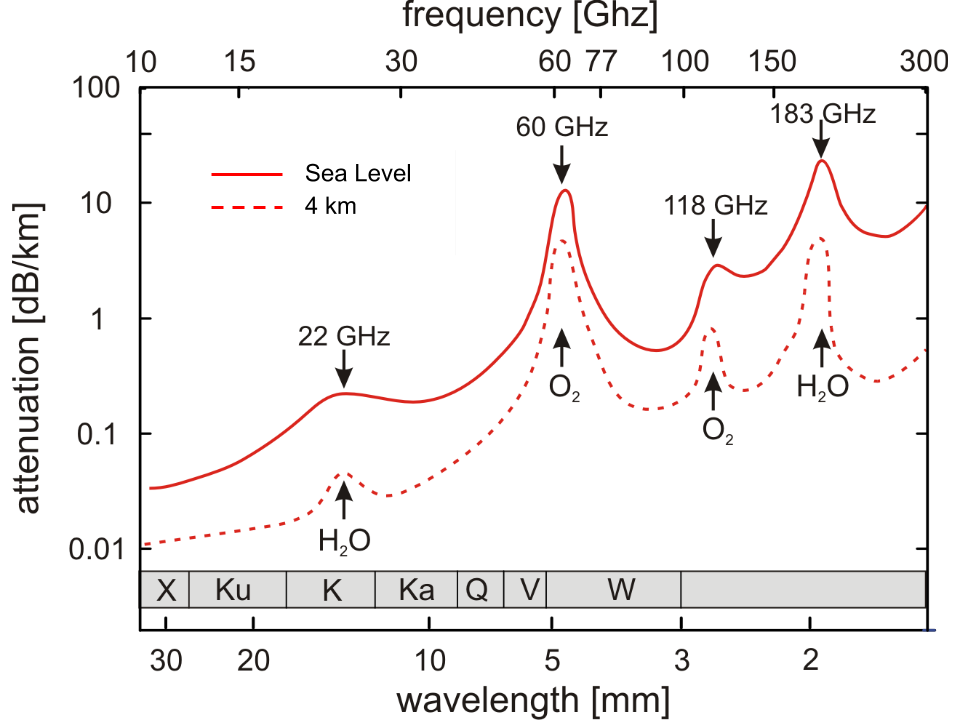
\includegraphics[width=0.45\textwidth]{Images/intro-atmospheric.png}
	\caption{\textbf{Atmospheric attenuation of radio waves by wavelength. Radio bandwidths are shown along the bottom horizontal axis.\cite{altshuler_comparison_1988}}}
	\label{fig:RadioAttenuation}
	\end{figure}
	
	Beyond the microwave band of electromagnetic radiation, the atmosphere becomes transparent again to light waves, posing another possible solution.
	Research into Earth-to-space high-bandwidth optical communication has been conducted by the NASA Jet Propulsion Lab since 2014.
	The Optical Payload for Lasercomm Science (OPALS) is an experimental optical communications system currently on-board the International Space Station that is being used to study the feasibility of such communications.
	The OPALS system uses a 1,550 nm 2.5W laser to communicate with a ground station on Earth, downlinking video data at 50 Mb/s. \cite{oaida_optical_2014}.
	Initial results have been promising, however there is a strict requirement on pointing accuracy of the laser, unlike radio and microwave signals. \cite{abrahamson_achieving_2015}
	
	\subsubsection*{Liquid Quenching}
	A technique that has been studied and even flight tested to good success is injecting a liquid such as water into the plasma flow field.
	The primary mechanism at work is electron recombination at or near the surface of water drops, thereby artificially reducing the electron number density in the plasma. %TODO citation needed.
	
	\subsubsection*{Magnetic Windows}
		
	\subsubsection*{Lorentz Windows}
	
	\subsubsection*{Stokes Waves}
	

	
	
\section{Prior Research} \label{sec:Prior}
	\subsection*{NASA RAM Studies}
	Radio wave attenuation in plasma sheaths and various methods of preventing it have been studied since at least the early 1960's.
	
	NASA's Radio Attenuation Measurement (RAM) project took place over nearly a decade from 1961 until 1970.
	Project RAM was one of the earliest sustained research efforts specifically targeted at the radio blackout problem for reentering space vehicles, and also the only known flight tests to date specifically to study the phenomenon and potential solutions to it.
	Since the scope of study was specifically targeted towards the radio blackout problem, and no other comparable flight testing has followed, data and findings from the RAM program are still cited in literature on the subject today.
	
	The RAM program consisted of a series of three flight test campaigns and eight flights total.
	The tests consisted of launching a reentry vehicle packed with plasma and radio diagnostic experiments on three and four-staged sounding rockets on a sub-orbital trajectory.
	The RAM A and B campaigns were comprised of four test flights which studied the reentry plasma sheath at a reentry velocity of 5.5 km/s (18,000 ft/s).\cite{huber_entry_1971}
	The two RAM A flights primarily studied aerodynamic shaping and magnetic window techniques, while the three RAM B flights studied water quenching and advanced study of the plasma sheath.
	The four RAM C flights reentered at 7.6 km/s (25,000 ft/s), which is comparable to low Earth orbit reentry velocities of around 8 km/s.
	The RAM C flights studied advanced plasma diagnostics as well as liquid quenching.\cite{huber_entry_1971}.
	
	\subsection*{Gemini Reentries}
	

\section{Active Solutions} \label{sec:Solutions}
	
\subsection*{Lorentz Windows}
\subsection*{Stokes Waves}

\bibliographystyle{ieeetr}
\bibliography{plasma_blackout}


\end{document}
